\section{Suggestions for improvement}\label{jiveSuggestions}

While exploring the features of \gls{jive}, a few issues regarding use and behavior were encountered.
None of these issues can be considered to be major, but they still expose a potential for improvement.
This section will point out some of the issues, and provide suggestions on what can be done to improve them.


\subsection{Visual changes to the diagrams}\label{jiveSuggestionsVisual}
%oppdage indre typer
In both diagrams, object instances are labeled with the name of the object type, and an instance-number, separated with a colon, e.g. `PersonPanel:1'.
While this provides the expected information, it is affected by the way Java handles the naming of anonymous inner types -- classes that are defined within another class, and not given a name by the developer.
Java automatically names these classes by appending a dollar sign and a identifying number to the name of the class they are defined within, e.g. `PersonPanel\$1'.
\gls{gui}-programs are written with several such classes to handle user input, each implementing a listener-interface of some kind, and they show up in the diagrams with their generated names, that do not reflect the purpose of the class.
The ability to detect an inner type with a generic name, and display the interface it implements, instead of its actual name, should help with this issue.
Among others, listener-heavy programs should become more understandable, as the kind of listeners in use will be clearly visible, removing the need to guess based on when they are invoked in the sequence-diagram.
\autoref{fig:contOving4ChangesLab} illustrates this as the change from part a to part b.


%koble listeners til det de lytter på
To further help users identify listeners, they could be visually linked to the objects they are listening to in the contour-diagram, making it clearly visible which object is being listened to by the different listeners.
\autoref{fig:contOving4ChangesLink} illustrates this change, along with the relabeled objects.
While the effect is possible to achieve by applying an appropriate filter, this filter must let a large amount of objects through, causing the diagrams to become cluttered and challenging to navigate.
On the other hand, the effect of the listener being triggered is clearly visible in the sequence diagram, and it is possible that this is easy enough to connect with a users interactions with a program, so that the addition of a specific link will not be necessary.
\begin{figure}[H]
	\centering
	\begin{subfigure}{\textwidth}
		\centering
		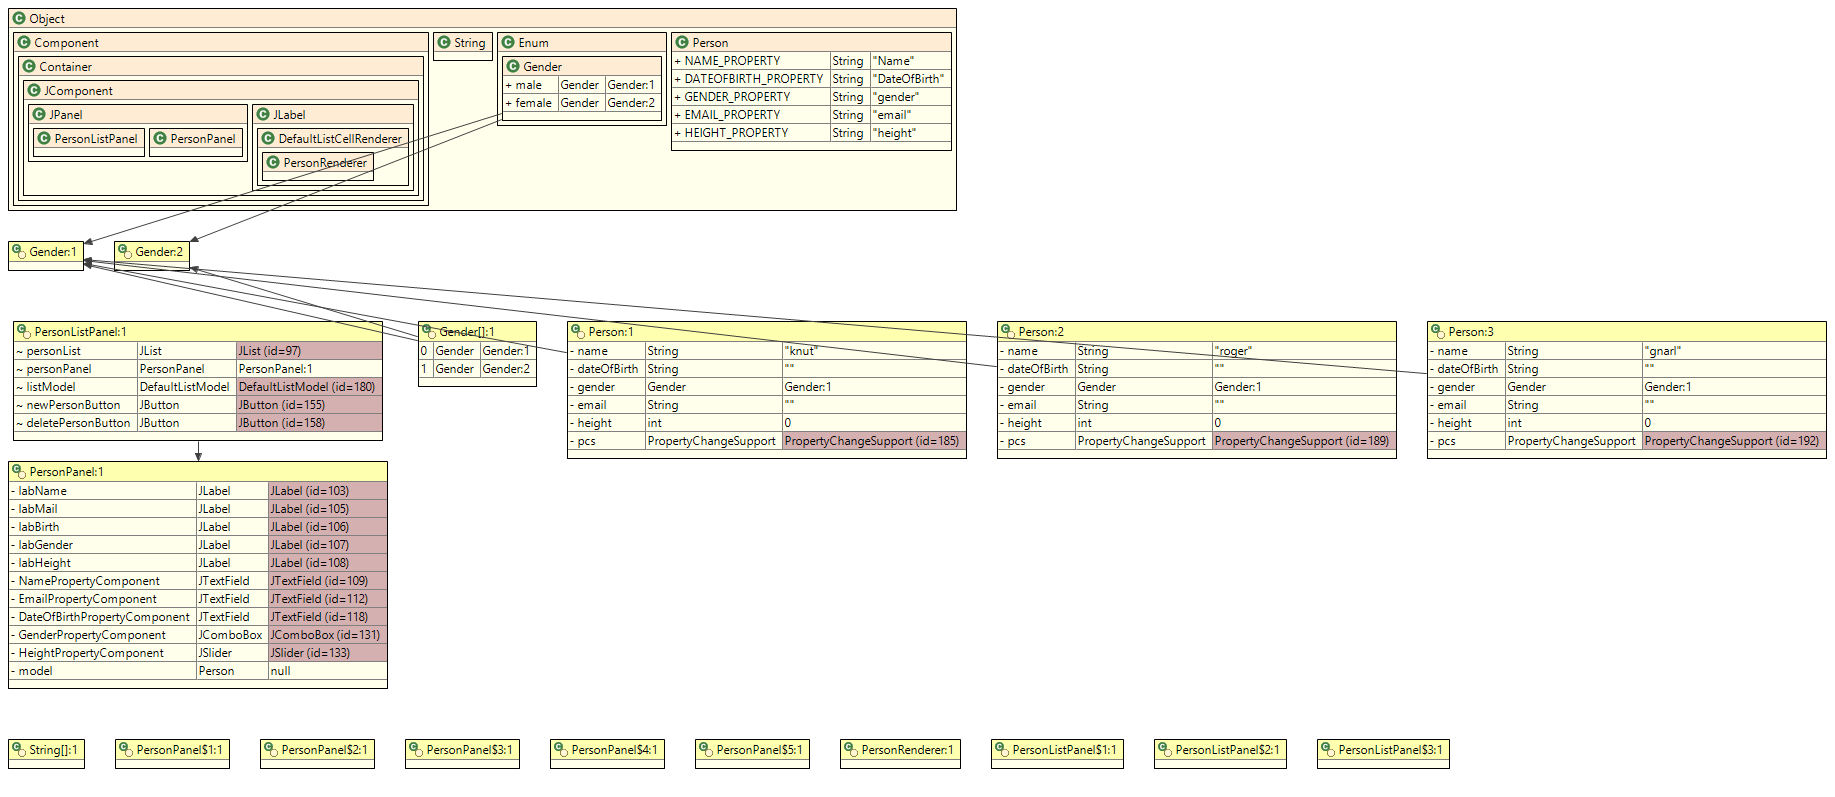
\includegraphics[width=\textwidth, trim= 0 0 36cm 26cm, clip]{MMI-Oving4-ObjectDiagInit}
		\caption{Original, cropped view of \autoref{fig:contOving4Init}}
		\label{fig:contOving4ChangesLabA}
	\end{subfigure}
	\begin{subfigure}{\textwidth}
		\centering
		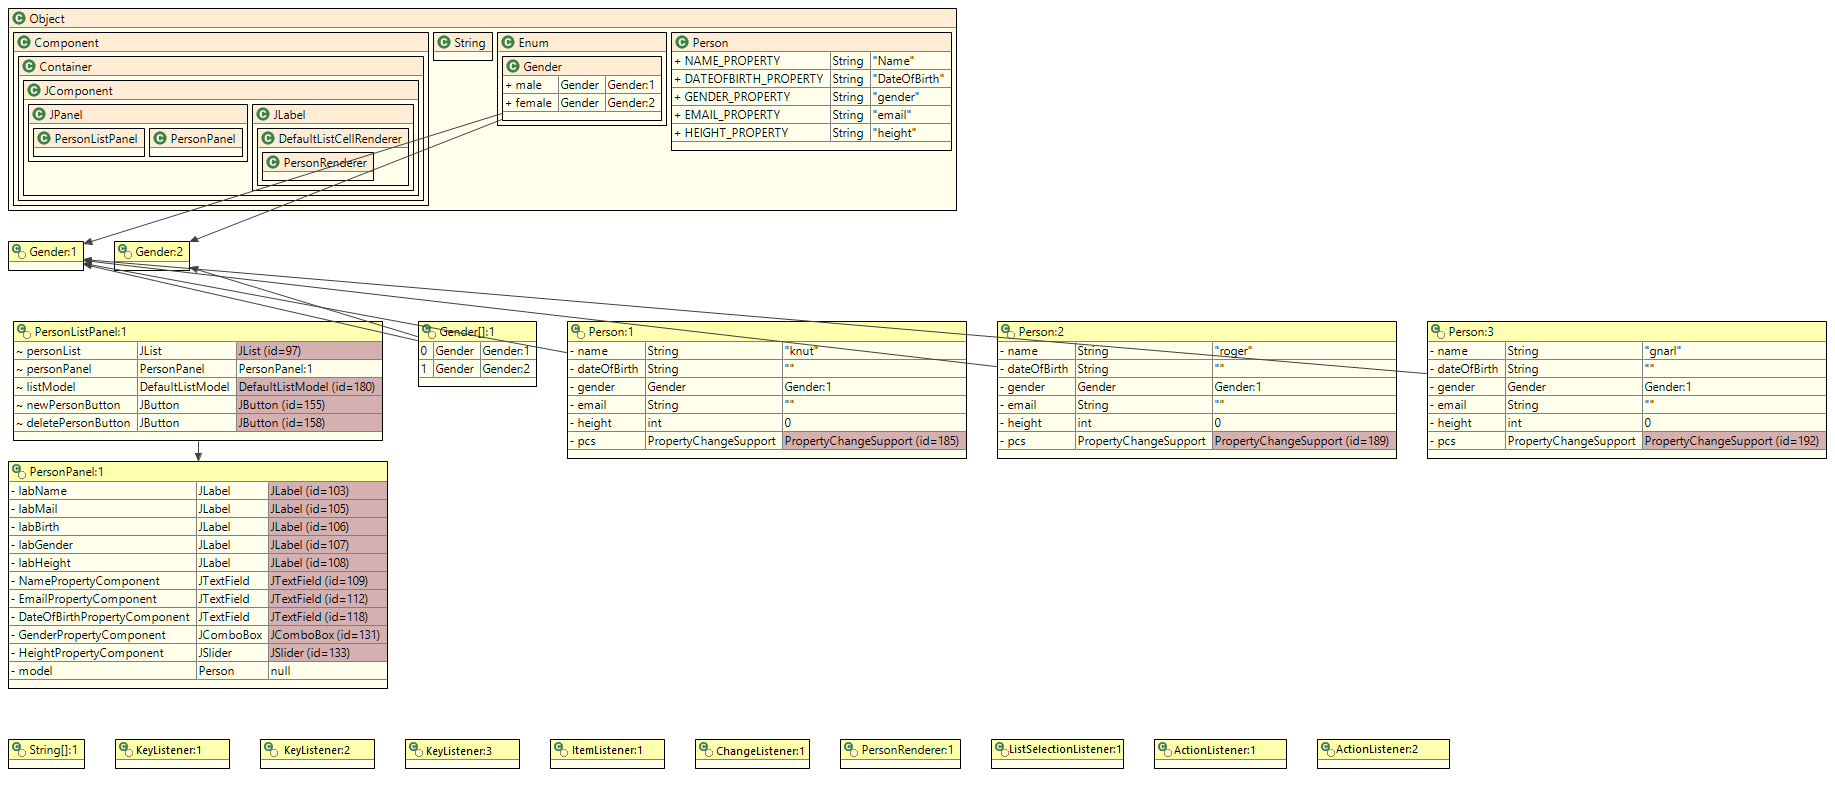
\includegraphics[width=\textwidth, trim= 0 0 27cm 19cm, clip]{MMI-Oving4-ObjectDiagInit-edit}
		\caption{Changed naming of anonymous inner types}
		\label{fig:contOving4ChangesLabB}
	\end{subfigure}
	\caption{comparison of the suggested label-changes to the diagrams}
	\label{fig:contOving4ChangesLab}
\end{figure}
%visualisere mvc-komonenter
A last visual change would be to attempt further identification of the components that make up an \gls{mvc}-architecture, and highlight them.
Being a change focusing solely on a specific architecture, it has to be possible to deactivate when not needed.
The major challenge with this feature is to find a way to identify the different components.
While listeners can usually be identified by their name, or by their implementation of certain interfaces, this is not necessarily the case for models and controllers.
A possible solution would be to require developers to follow a certain naming scheme, but this would still have a risk of false positives -- leading to incorrect diagrams, and adoption of such a scheme with the sole purpose of using a special tool, is not something to expect.
The highlighting could be done by adding colored frames to the identified objects, or by adding an icon indicating the role of a given object.
Not as big of a challenge, this does pose the problem of maintaining the the readability of the diagrams, and not making them harder to read due to the added elements.


\begin{figure}[H]
	\centering
	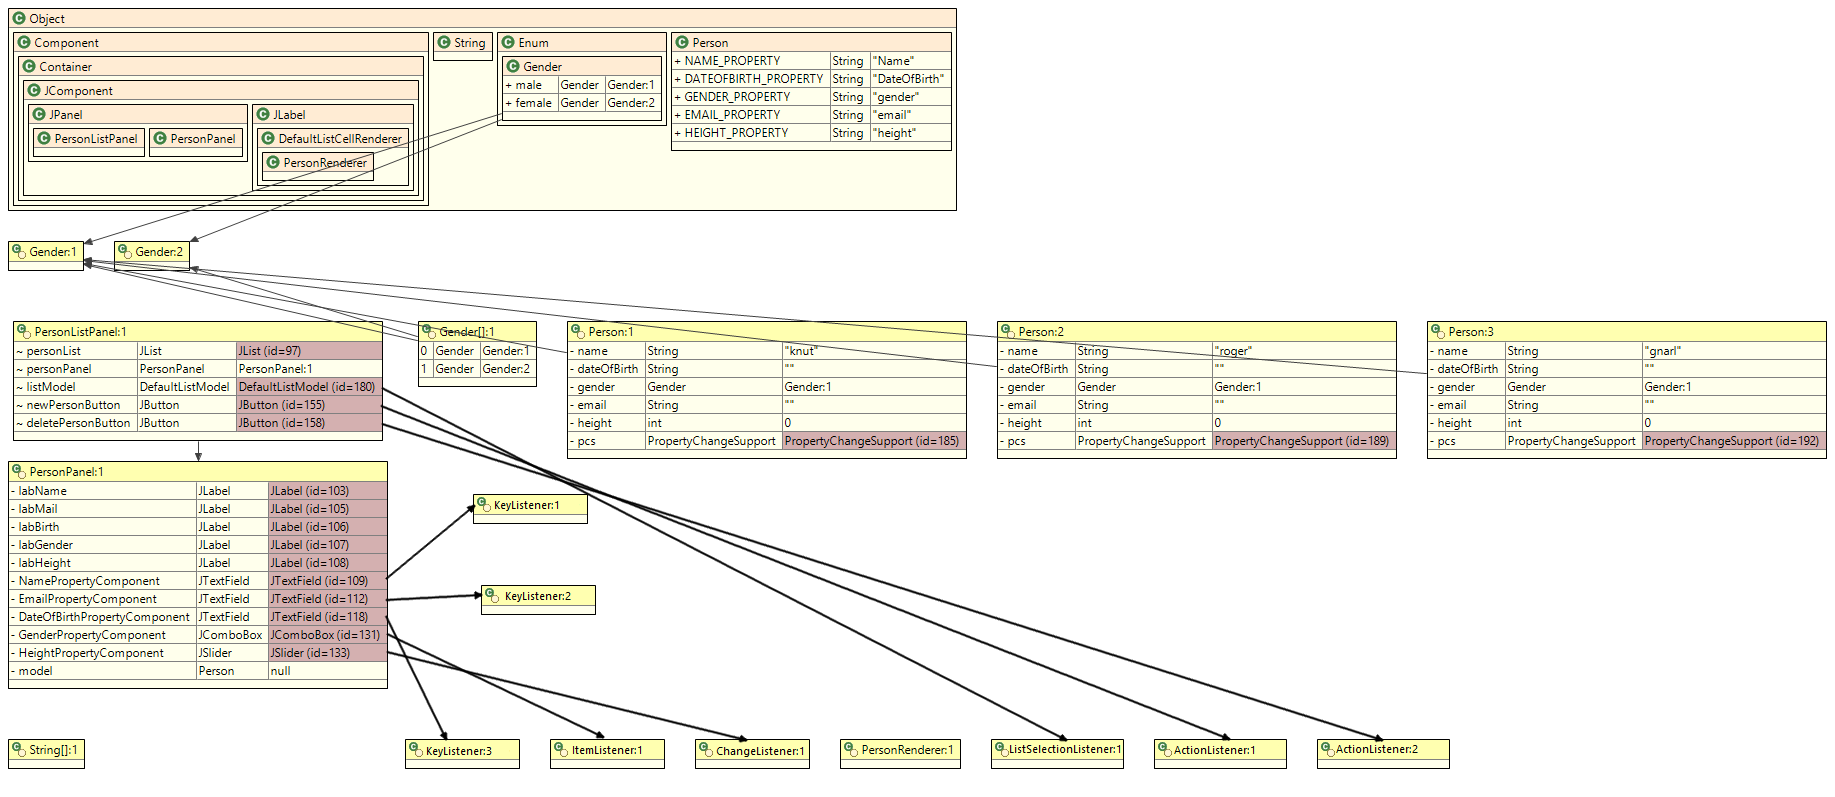
\includegraphics[width=\textwidth, trim= 0 0 0 0, clip]{MMI-Oving4-ObjectDiagInit-edit3}
	\caption{Listeners are relabeled, and connected to the objects they listen to. The illustration is based on \autoref{fig:contOving4Init}}
	\label{fig:contOving4ChangesLink}
\end{figure}


\subsection{Functional changes}\label{jiveSuggestionsFunctional}
%bruker-tilpasning av diag
Both diagrams can easily grow to sizes that make them hard to navigate and to get an overview of.
While the contour diagram offers different presentation modes, by for instance only showing objects, and not their data-fields, the sequence diagram offers fewer options.
Collapsing parts of the diagrams do help in reducing the amount of information shown, and thus ease the interpretation of the diagram, but there are still some issues that result from how the diagram is drawn.
Firstly, there is currently no method of vertically compressing the sequence diagram, resulting in long sequences with no visible interaction if that sequence has already been collapsed, or if there are a lot of filtered events occurring within the lifeline of an object.
There is an ongoing development to solve this, by substituting an event-pattern with a single new event, and thus reducing the vertical size of the diagram.
If this technique is applied when using the existing horizontal collapse, the diagram should shrink in both directions.


The other issue is a consequence of having the objects at the top of the sequence diagram added in the order in which they are used.
This is generally a good way to order the objects, especially when considering the start-up sequence of a program, which is then displayed in a well organized way.
Where this approach becomes problematic, is when the newer objects start interacting with the older ones, causing the lines that indicate method calls to cross over parts of the diagram, and often going back and forth.
This problem is illustrated in \autoref{fig:seqOving4CrossLines}, where a listener triggers activity in an older part of the program.


\begin{figure}[H]
	\centering
	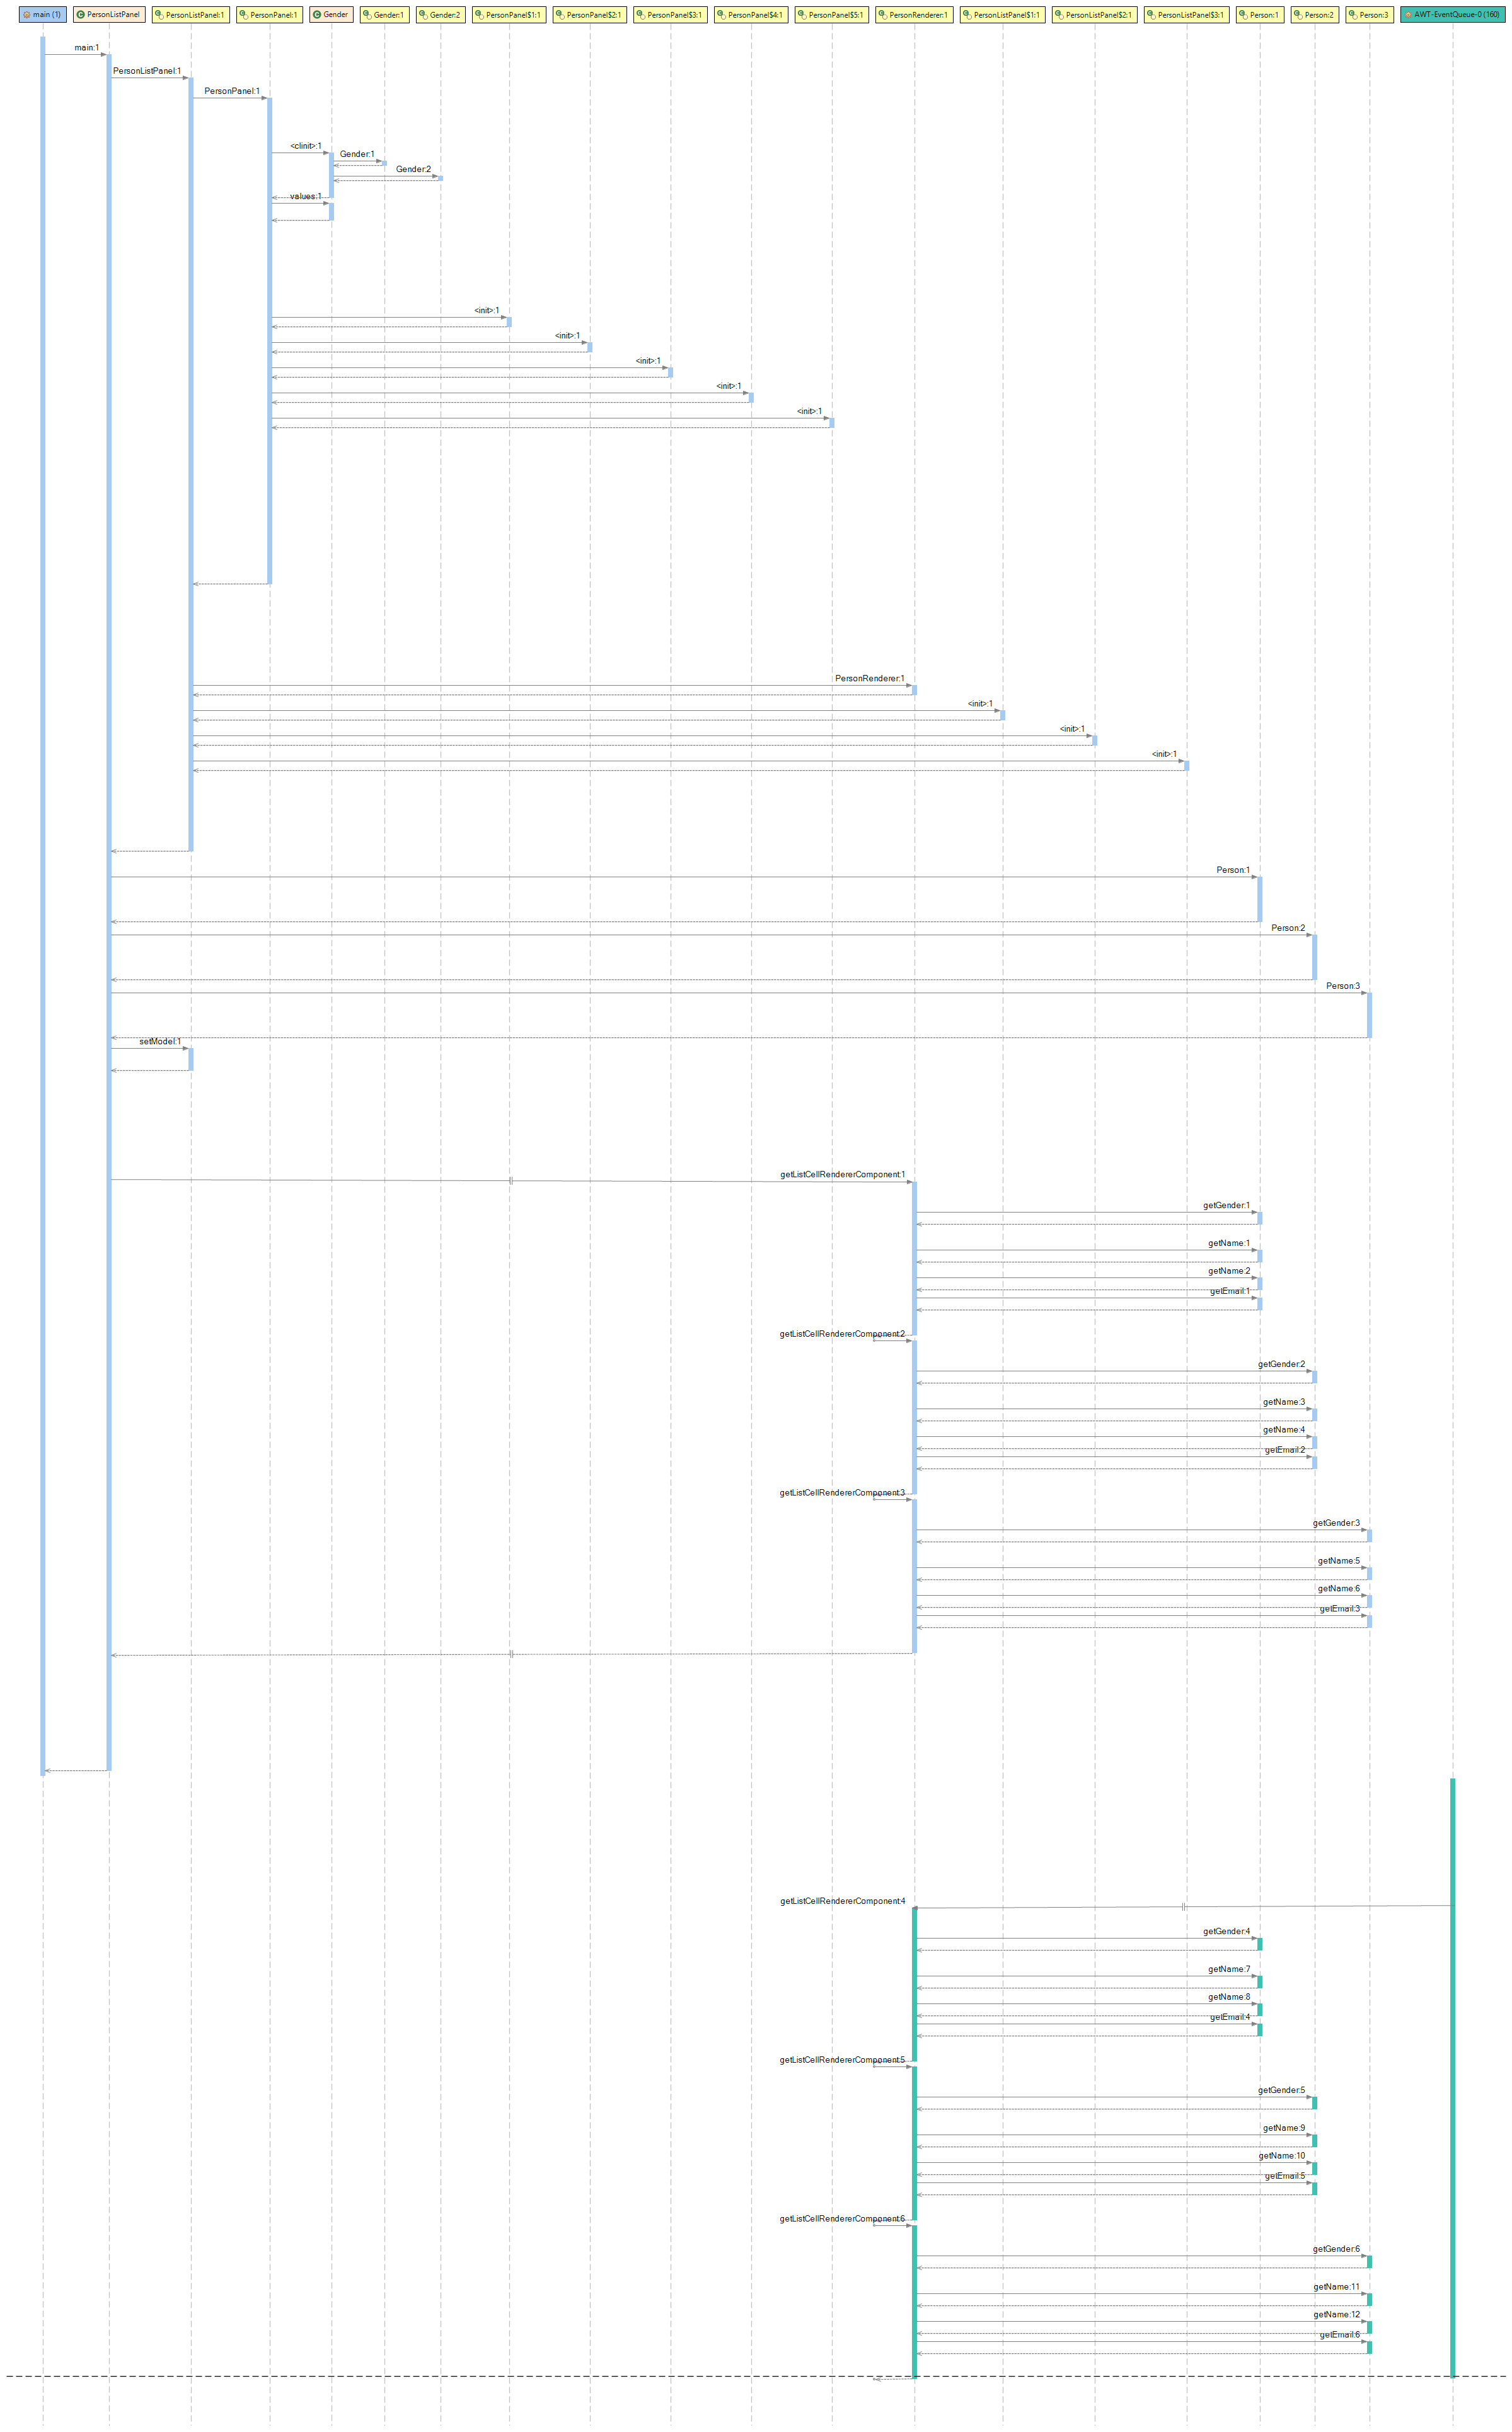
\includegraphics[width=\textwidth, trim= 45cm 7cm 0cm 103cm, clip]{MMI-Oving4-SequenceDiagInit}
	\caption{A section of a larger sequence diagram, showing method calls crossing several unrelated lifelines}
	\label{fig:seqOving4CrossLines}
\end{figure}


%isolert visning
In some cases, the amount of unrelated lifelines that surround a sequence becomes so large, that fitting the entire sequence within the view of a single screen becomes impossible without zooming out, and thus rendering the text unreadable.
Scrolling sideways to follow consecutive events is not ideal, and can potentially be disorienting.
This could be solved by allowing users to view such a sub-sequence in a separate, isolated environment, with the objects lined up in the order in which they are used, as illustrated in \autoref{fig:seqOving4IsolatedMock}.


\begin{figure}[H]
	\centering
	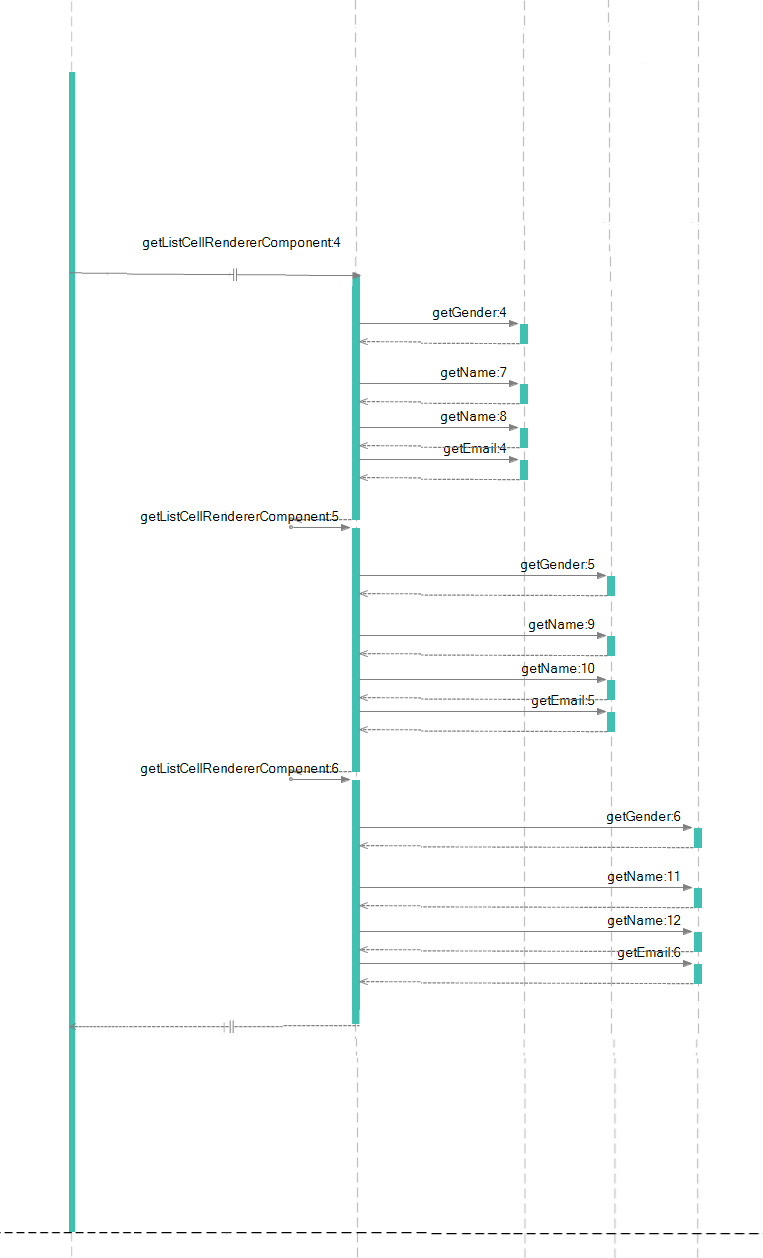
\includegraphics[height =.5\paperheight, trim= 0cm 5cm 0cm 5cm, clip]{MMI-Oving4-SequenceDiagInit-isolatedEventsMock}
	\caption{An example of how \autoref{fig:seqOving4CrossLines} might look in the isolated view}
	\label{fig:seqOving4IsolatedMock}
\end{figure}


%filter-endringer
The filter operates by excluding unwanted elements from the trace-log, and only takes a list of elements to exclude as input.
While this simplifies the internal operation, and makes it easy for users to understand, it also makes it hard to build a more fine grained filter, where, for instance, a package containing several sub-packages is excluded, but one of those sub-packages is not.
The current way to achieve this is to individually list each of the sub-packages that are excluded, while omitting the one that should be included.
This results in a potentially large list of packages, and will take an unnecessary amount of work to add to the filter.
By instead allowing the users to add the one package to be included, and using both a list of inclusions and a list of exclusions to build the filter, the amount of work for the user is significantly reduced, while maintaining readability.


Changing the filter is currently done by adding or removing one entry at a time, making large changes time consuming and prone to spelling errors.
Since the filters are stored in the files Eclipse uses to describe how to launch a program, directly modifying these files is a possible work-around for making large changes, but they require Eclipse to be restarted to have any effect.
These files are also hidden within the configuration folders that Eclipse uses, making them hard to find without instructions.
Having an easier way of swapping, or making large changes to filters, would likely increase the use of custom filters, and would enable the distribution of pre-made filters, designed for specific purposes.
This feature could be extended further, to include multiple default filters that a user could select from when running a program.


%søk
The ability to search through all the events is a potentially useful feature, depending on the scenario in which \gls{jive} is used.
When merely getting an overview of a program, it is likely not needed at all, but for debugging purposes, it has a clear use as a way of finding specific events.
It is unfortunately very strict in its interpretation of the search terms, being both case-sensitive, and requiring full class names, including the package the class is contained within.
It is assumed that this behavior was chosen in order to give an accurate, and limited set of results, instead of risking a large amount of false positives.
On the other hand, this behavior goes against the expectations set by most search providers in other areas, and can lead to confused users, that may, at worst, consider the search to be non-functional.
By relaxing the search criteria to not be case sensitive, and to allow partial matches, the usage of this feature would be less confusing, and still allow the users to narrow their results by being more specific with their search-terms.


%batch-kjøring av større prog? automatisert ui-interaksjon
Despite the measures that have been taken to reduce the performance impact of \gls{jive}, it will always be possible to create a scenario where the analyzed program will take a significant amount of time to run.
For instance when testing a larger project.
For non-interactive programs, this is only a matter of waiting for results.
But in order to get the desired results from an interactive program, it becomes necessary to check back regularly in order to provide the correct input.
Integrating automation tools that trigger pre-defined inputs when they detect that the program is waiting for interaction, would go a long way towards solving this.
A user could first run a session without \gls{jive}, and record the desired interactions.
These interactions would then be fed into the automaton tool and played back during the \gls{jive}-run.
As this kind of feature is not required for the exercises given during the \gls{hci}-course, it is not prioritized above the other mentioned changes.




